\documentclass{article}

\usepackage{ctex}
\usepackage{listings}
\usepackage[framed,numbered,autolinebreaks,useliterate]{mcode}
\usepackage{geometry}
\usepackage{multirow}
\usepackage{graphicx}
\usepackage{amsmath}
\usepackage{float}
\geometry{a4paper, scale=0.8}

\title{数学实验实验报告}
\author{ZhaohengLi 2017050025\\cainetatum@foxmail.com\\15801206130}

\begin{document}
\maketitle
\section{实验目的}
\begin{itemize}
	\item{掌握 MATLAB 优化工具箱的基本使用方法,对不同算法进行分析和比较;}
	\item{练习使用无约束方法建立和求解实际问题模型。}
\end{itemize}


\section{CH7-T5 原子位置}

\subsection{模型建立}
首先建立原子位置的平面直角坐标系,并假设第一个原子的位置在平面直角坐标系的原点位置,这种假设并不影响各个原子的相对位置关系。

设第i个原子的位置为$(x_i,y_i)\quad (i=2,3,\cdots,25)$,且第i个原子和第j个原子的距离为$d_{ij}$。在此情况下,问题转化为求得最优的坐标集合$(x_i,y_i)$,使得题目中给出的距离关系尽量满足。

设题目中所有给定的距离关系的点对坐标集合为M,以满足条件的欧式距离作为误差衡量标准,给出下列无约束优化目标。

$$min\sum_{(i,j)\in M}[(x_i-x_j)^2+(y_i-y_j)^2-d_{ij}^2]^2$$

最终各个原子的位置关系便可以通过直角坐标系的坐标进行表示了。

\subsection{算法设计}
根据题目中所给数据,这是一个 48 变量的优化问题,应尝试采用 MATLAB 工具箱中的 fminunc工具求解,并使用 BFGS、 DFP 和最速下降法进行比较,取使目标函数最小的变量值作为最终结果。此外,还可以调整收敛的精度,进一步提高准确性。

MATLAB代码如下:

\begin{lstlisting}
%% Global Variables
global M;
M = [4, 1, 0.9607; 12, 1, 0.4399; 13, 1, 0.8143;
    17, 1, 1.3765; 21, 1, 1.2722; 5, 2, 0.5294;
    16, 2, 0.6144; 17, 2, 0.3766; 25, 2, 0.6893;
    5, 3, 0.9488; 20, 3, 0.8000; 21, 3, 1.1090;
    24, 3, 1.1432; 5, 4, 0.4758; 12, 4, 1.3402;
    24, 4, 0.7006; 8, 6, 0.4945; 13, 6, 1.0559;
    19, 6, 0.6810; 25, 6, 0.3587; 8, 7, 0.3351;
    14, 7, 0.2878; 16, 7, 1.1346; 20, 7, 0.3870;
    21, 7, 0.7511; 14, 8, 0.4439; 18, 8, 0.8363;
    13, 9, 0.3208; 15, 9, 0.1574; 22, 9, 1.2736;
    11, 10, 0.5781; 13, 10, 0.9254; 19, 10, 0.6401;
    20, 10, 0.2467; 22, 10, 0.4727; 18, 11, 1.3840;
    25, 11, 0.4366; 15, 12, 1.0307; 17, 12, 1.3904;
    15, 13, 0.5725; 19, 13, 0.7660; 15, 14, 0.4394;
    16, 14, 1.0952; 20, 16, 1.0422; 23, 16, 1.8255;
    18, 17, 1.4325; 19, 17, 1.0851; 20, 19, 0.4995;
    23, 19, 1.2277; 24, 19, 1.1271; 23, 21, 0.7060;
    23, 22, 0.8052];

%% CAl
% x0 = ones(48,1);
x0 = -1+2 * rand(48, 1);
opt = optimset('HessUpdate', 'bfgs', 'MaxFunEvals', 1000000, 'MaxIter', 10000, 'LargeScale', 'off');
% opt = optimset('HessUpdate', 'dfp', 'MaxFunEvals', 1000000, 'MaxIter', 10000);
% opt = optimset('HessUpdate', 'steepdesc', 'MaxFunEvals', 1000000, 'MaxIter', 10000);
[xres, vres, exitr, outr] = fminunc(@atomdis, x0, opt);
y = zeros(500, 1);

for i = 1:1:500
    x0 = -1+2 * rand(48, 1);
    opt = optimset('HessUpdate', 'bfgs', 'MaxFunEvals', 1000000, 'MaxIter', 10000, 'LargeScale', 'off');
    [xres, vres, exitr, outr] = fminunc(@atomdis, x0, opt);
    y(i) = vres;
end
%% Plot
scatter(y(1:2:47),y(2:2:48))
scatter(xres(1:2:47),xres(2:2:48))

%% Function

function y = atomdis( x )
    global M;
    y = 0;
    for t = 1:length(M)
        i = M(t, 1);
        j = M(t, 2);
        dij = M(t, 3);
        
        if i == 1 
            x_i = 0;
            y_i = 0;
        else
            x_i = x(2*(i-1)-1);
            y_i = x(2*(i-1));
        end
        
        if j == 1 
            x_j = 0;
            y_j = 0;
        else
            x_j = x(2*(j-1)-1);
            y_j = x(2*(j-1));
        end
        
        y = y + ((x_i - x_j)^2 + (y_i - y_j)^2 - dij * dij) ^ 2;
    end
end
\end{lstlisting}

\subsection{计算结果}
在计算条件设置方面,实验中使用了BFGS、 DFP和最速下降法三种方法进行计算,最大迭代次数选择$10^4$,最大方程求值次数选择$10^6$,初始值选择$0$,$(0,4)$内随机值或$(-1,1)$内随机值三种方式。

因为在进行实验之前进行了几组预实验,发现大部分用例和算法在迭代$10^4$次,函数调用$10^6$次内计算得出结果,因此在本实验中不再对迭代次数、函数调用次数这两参量进行讨论,故实验中最大迭代次数选择$10^4$,最大方程求值次数选择$10^6$。

算法表现结果为:
\begin{table}[H]
\centering
\begin{tabular}{|l|l|l|l|l|l|}
\hline
方法    & 初始值设置    & 迭代次数 & 函数调用次数 & 求得函数值  & 用时(s)   \\ \hline
Steep & 1      & 710    & 104664   & 2.6499 & 1.7 \\ \hline
BFGS  & 1      & 152    & 7978     & 0.0482 & 0.2  \\ \hline
DFP   & 1      & 2484   & 122549   & 0.1224 & 0.3  \\ \hline
Steep & (0.4)  & 6799   & -        & 0.0656 & 4.1  \\ \hline
BFGS  & (0,4)  & 371    & 18522    & 0.0348 & 0.3  \\ \hline
DFP   & (0,4)  & -      & 490098   & 0.3899 & 0.6  \\ \hline
Steep & (-1,1) & 6800   & -        & 0.0672 & 4.0  \\ \hline
BFGS  & (-1,1) & 266    & 13328    & 0.0159 & 0.2  \\ \hline
DFP   & (-1,1) & 3655   & 179144   & 0.0269 & 0.4  \\ \hline
\end{tabular}
\end{table}
图中标‘-’表示超出最大次数,从表格中可以得出看出:

在迭代次数和函数调用次数方面,最速下降法所需要的迭代次数和函数调用次数在大部分情况下是最多的,而且还经常会超过设定的阈值,远远大于其他算法。同时可以看到BFGS算法使用次数最少。

在计算结果上看,BFGS算法表现最好,在三次实验中均取得了最好的成绩。

在计算用时方面,同样是BFGS算法表现最好,DFP表现稍逊于BFGS,而最速下降法表现十分不好,用时远远大于其他两算法。

在初始值设定方面来看,设定于$(-1,1)$内随机值表现较好,我认为原因有两点。题目中给出的原子对距离分布在$(0,2)$内,选取区间长度为2内的随机值会取得更好的初值计算条件;由于我们设定了第一个原子在坐标原点,因此以坐标原点为中心对称的随机值区间会取得较好的计算结果。

通过上述的实验,我重新选取了计算条件,使用BFGS算法并令初值为分布在在$(-1,1)$区间的随机数,尝试了500次,统计每次计算所得的函数值做成下图:

\begin{figure}[H]
    \centering
    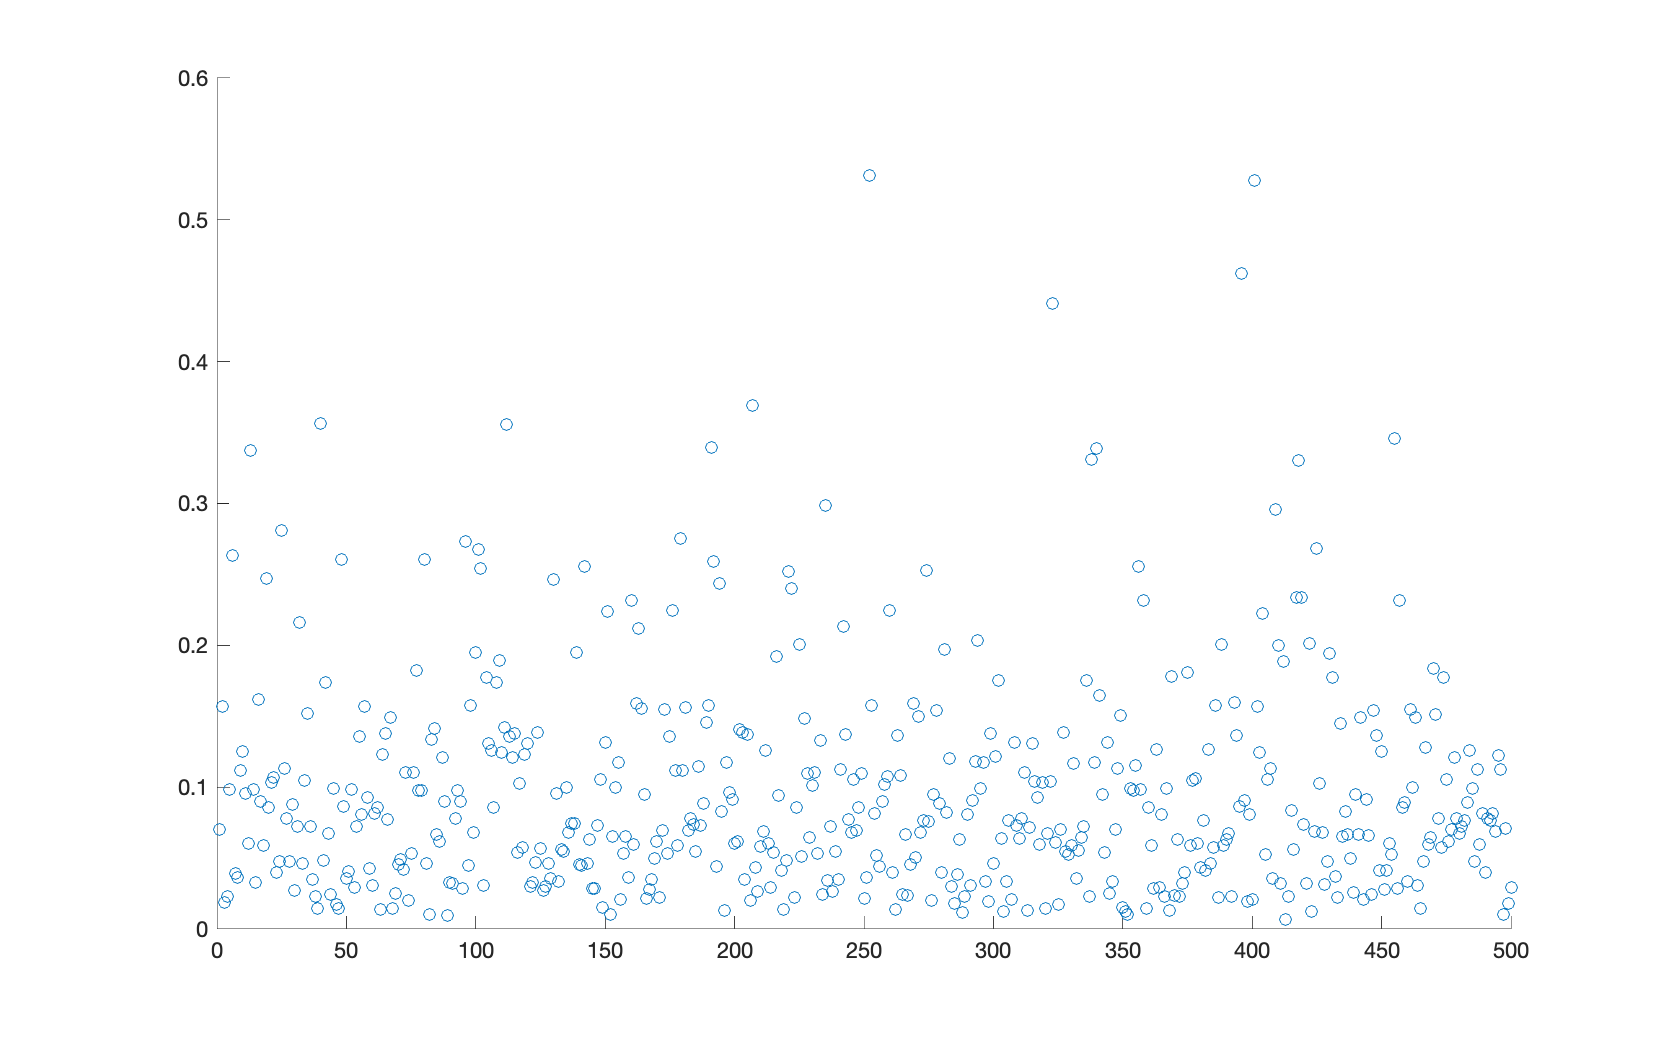
\includegraphics[width=0.9\textwidth]{pic1.png}
    \caption{500次不同初始值计算所得的最小函数值}
\end{figure}
从图中可以看出,初始值对最终结果的影响非常大,不同初值得到的结果很不一样,因此我们要多多尝试不同的初值。

最终使用BFGS算法取一个目标函数值最小的x作为最终输出$(f_{min}=0.012)$。最终求得的各个原子坐标位置如下图所示:

\begin{figure}[H]
    \centering
    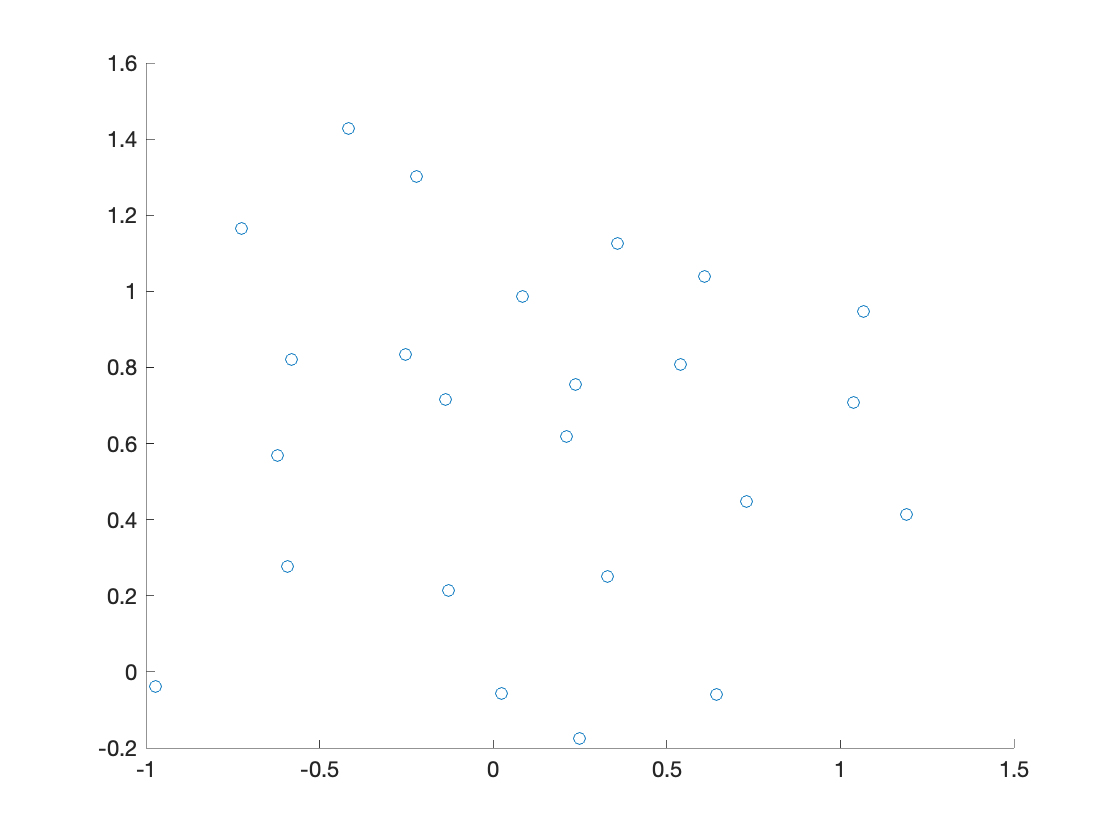
\includegraphics[width=0.9\textwidth]{pic3.png}
    \caption{原子位置}
\end{figure}
\subsection{结果分析}
根据上述使用不同方法和不同初值进行分析比较,可以看出在求解本题的过程中,使用 BFGS 公式的拟牛顿法能够以较少的迭代次数和函数求值次数得到较优的函数值,相比于 DFP 公式和最速下降法表现更好。在初值的选取方面,能够看出初值对于方法的函数求值次数和最终找到的是否为全局最优解关系很密切。在图中可以清楚地看到这一点。在选择某 些初始值时,能够求得全局的最优值,而有些初始值则可能误导算法进入局部最优解并停止迭代。因此要多尝试不同的初值求得最优结果。

\section{CH7-T8 用药方案}
\subsection{模型建立}
问题可以转换成利用数据拟合方程:
$$c(t)=\frac dv\frac{k_1}{k_1-k}(e^{-kt}-e^{-k_1t})$$

可以看出这个方程是非线性的,因此这是一个非线性最小二乘拟合的问题,故可以选用MATLAB中的lsqcurvefit函数求解。

\subsection{模型求解}
MATLAB代码如下:

\begin{lstlisting}
%% Global Variables
t = [0.083, 0.167, 0.25, 0.5, 0.75, 1, 1.5, 2.25 3, 4, 6, 8, 10, 12];
c = [10.9, 21.1, 27.3, 36.4, 35.5, 38.4, 34.8, 24.2, 23.6, 15.7, 8.2, 8.3, 2.2, 1.8];

%% Cal
x0 = [1,1,0];
x = lsqcurvefit(@medicine,x0,t,c);

%% Function

function c = medicine(x, t)
    c = x(1)*x(2)/(x(2)-x(3))*(exp(-x(3)*t)-exp(-x(2)*t));
end
\end{lstlisting}

得到的结果为$k_1=3.6212,k=0.2803,b=46.8275$,另外得出$norm=34.2317$,得出药物释放曲线图如下:


\begin{figure}[H]
    \centering
    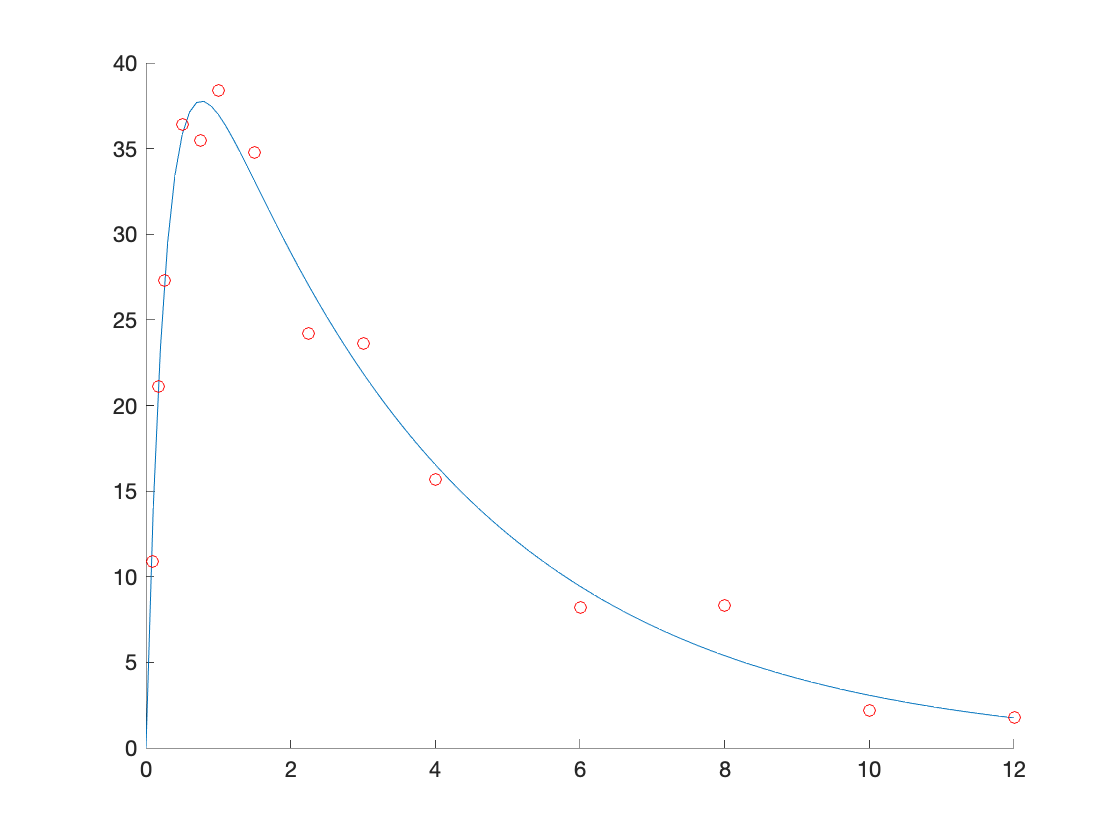
\includegraphics[width=0.9\textwidth]{pic4.png}
    \caption{药物释放曲线}
\end{figure}


\subsection{模型分析}
接下来变化初值来实验,得到如下结果:

\begin{table}[H]
\centering
\begin{tabular}{|l|l|l|l|}
\hline
初始值          & 迭代次数 & norm & 求得函数值            \\ \hline
(1,1,0)      & 24   & 34.2 & 46.82,3.621,0.28 \\ \hline
(1,2,1)      & 24   & 34.2 & 46.82,3.621,0.28 \\ \hline
(1,2,40)     & 9    & 34.2 & 46.82,3.621,0.28 \\ \hline
(1,2,100)    & 9    & 34.2 & 46.82,3.621,0.28 \\ \hline
(1,2,200)    & 10   & 34.2 & 46.82,3.621,0.28 \\ \hline
(3,0.3,50)   & 4    & 34.2 & 46.82,3.621,0.28 \\ \hline
(20,10,50)   & 22   & 34.2 & 46.82,3.621,0.28 \\ \hline
(200,100,50) & 26   & 34.2 & 46.82,3.621,0.28 \\ \hline
\end{tabular}
\end{table}
可以看到,在本题中,初值对于最终结果的影响不大,但是初值的选择影响着函数的迭代次数,合适的初值可以较快的得到结果。

\section{CH8-T6 投资}
\subsection{模型建立}
设公司购进了A证券$x_A$万元,B证券$x_B$万元,C证券$x_C$万元,D证券$x_D$万元,E证券$x_E$万元,考虑纳税情路,则总收益为:

$$z=p_Ax_A+0.5p_Bx_B+0.5p_Cx_C+0.5p_Dx_D+p_Ex_E$$

其中,$p_A,\cdots,p_E$代表各个证券的税前收益。系数0.5代表$50\%$的纳税。

约束条件(1)可以表示为:

$$x_B+x_C+x_D\geq 400$$

约束条件(2)可以表示为:

$$\frac{l_Ax_A+l_Bx_B+l_Cx_C+l_Dx_D+l_Ex_E}{x_A+x_B+x_C+x_D+x_D+x_E}\leq1.4$$

化简为:

$$(1.4-l_A)x_A+(1.4-l_B)x_B+(1.4-l_C)x_C+(1.4-l_D)x_D+(1.4-l_E)x_E\geq0$$

其中,$l_A,\cdots,l_E$代表着各个证券的税前收益。

约束条件(3)可以表示为:

$$\frac{y_Ax_A+y_Bx_B+y_Cx_C+y_Dx_D+y_Ex_E}{x_A+x_B+x_C+x_D+x_D+x_E}\leq5$$

化简为:

$$(5-y_A)x_A+(5-y_B)x_B+(5-y_C)x_C+(5-y_D)x_D+(5-y_E)x_E\geq0$$

其中,$y_A,\cdots,y_E$代表着各个证券的税前收益。

对于第一问,需要增加条件:

$$x_A+x_B+x_C+x_D+x_E\leq 1000$$

对于第二问,假设借用的金额为k万元,需要增加条件:

$$k\leq100$$

且需要修正目标函数为:

$$z=p_Ax_A+0.5p_Bx_B+0.5p_Cx_C+0.5p_Dx_D+p_Ex_E-0.0275k$$

同时增加约束:

$$x_A+x_B+x_C+x_D+x_E\leq k+1000$$

\subsection{算法设计}
根据上述模型分析可知,所有约束均为线性不等式,目标函数也为线性,符合线性规划 的一般形式,因此使用 LINGO 的 Linear Programming 功能直接进行求解即可。
对于第 (3) 问的目标函数参数敏感性分析,可以通过 LINGO 的 Prices\& Ranges命令 进行分析。

LINGO代码如下:

(1)
\begin{lstlisting}
MODEL:
Title Stock Investment;
sets:
sn/1..5/: p, l, y, x, cutoff;
endsets
data:
p = 0.043 0.054 0.05 0.044 0.045; l = 2 2 1 1 5;
y = 9 15 4 3 2;
cutoff = 1 0.5 0.5 0.5 1;
enddata
[OBJECTIVE] max = @sum(sn: cutoff * p * x);
[CONS1] x(2) + x(3) + x(4) >= 400;
[CONS2] @sum(sn: (1.4 − l) * x) >= 0;
[CONS3] @sum(sn: (5 − y) * x) >= 0;
[T1CONS] @sum(sn: x) <= 1000;
END
\end{lstlisting}

(2)
\begin{lstlisting}
MODEL:
Title Stock Investment;
sets:
sn/1..5/: p, l, y, x, cutoff;
endsets
data:
p = 0.043 0.054 0.05 0.044 0.045; l = 2 2 1 1 5;
y = 9 15 4 3 2;
cutoff = 1 0.5 0.5 0.5 1;
enddata
[OBJECTIVE] max = @sum(sn: cutoff * p * x) − 0.0275 * k;
[CONS1] x(2) + x(3) + x(4) >= 400;
[CONS2] @sum(sn: (1.4 − l) * x) >= 0;
[CONS3] @sum(sn: (5 − y) * x) >= 0;
[T2CONS1] @sum(sn: x) <= 1000 + k;
[T2CONS2] k <= 100;
END
\end{lstlisting}

\subsection{计算结果分析}
\subsubsection{第一问}
LINGO 输出的结果使用了 LP 模型,求解器迭代次数为 3,最终结果如下表所示:
\begin{table}[H]
\centering
\begin{tabular}{|l|l|l|}
\hline
变量 & 最优取值   & 减少费用   \\ \hline
xA & 218.18 & 0(基变量) \\ \hline
xB & 0      & 0.03   \\ \hline
xC & 736.36 & 0(基变量) \\ \hline
xD & 0      & 0.0006 \\ \hline
xE & 45.45  & 0(基变量) \\ \hline
\end{tabular}
\end{table}

另外,根据 LINGO 的松弛变量输出,还可知条件 CONS2、CONS3、T1CONS的松弛变量 为 0,说明这几个约束起了作用。

最优目标函数值为 29.836。

\subsubsection{第二问}

LINGO 输出的结果使用了 LP 模型,求解器迭代次数为 3,最终结果如下表所示:

\begin{table}[H]
\centering
\begin{tabular}{|l|l|l|}
\hline
变量 & 最优取值   & 减少费用   \\ \hline
xA & 240 & 0(基变量) \\ \hline
xB & 0      & 0.03   \\ \hline
xC & 810 & 0(基变量) \\ \hline
xD & 0      & 0.0006 \\ \hline
xE & 50  & 0(基变量) \\ \hline
k  & 100    & 0(基变量) \\ \hline
\end{tabular}
\end{table}


另外,根据 LINGO 的松弛变量输出,还可知条件 CONS2、CONS3、T2CONS1、T2CONS2的 松弛变量为 0,说明这几个约束起了作用。

最优目标函数值为 30.07。


\subsubsection{第三问}

针对第 (1) 问的 Range 分析,可以得到的分析如下:

\begin{table}[H]
\centering
\begin{tabular}{|l|l|l|l|}
\hline
Variable                                                       & Current Coefficient                                                                                                   & Allowable Increase                                                                                                    & Allowable Decrease                                                                                          \\ \hline
\begin{tabular}[c]{@{}l@{}}x1\\ x2\\ x3\\ x4\\ x5\end{tabular} & \begin{tabular}[c]{@{}l@{}}0.4300000E−01\\ 0.2700000E−01\\ 0.2500000E−01\\ 0.2200000E−01\\ 0.4500000E−01\end{tabular} & \begin{tabular}[c]{@{}l@{}}0.3500000E−02\\ 0.3018182E−01\\ 0.1733333E−01\\ 0.6363636E−03\\ 0.5200000E−01\end{tabular} & \begin{tabular}[c]{@{}l@{}}0.1300000E−01\\ INFINITY\\ 0.5600000E−03\\ INFINITY\\ 0.1400000E−01\end{tabular} \\ \hline
\end{tabular}
\end{table}

当证券 A 的税前收益增加 0.2\% 的时候,在变量 X(1)的增加允许范围 0.35\% 之内,所 以投资可以不改变;当证券 C 税前收益减少 0.2\% 的时候,不在变量 X(3)的减少允许范围 0.056\% 之内,所以投资应该改变。

\subsection{结论}

若该经理有 1000 万元资金,应该投资 A 证券 218.18 万元、投资 C 证券 736.36 万元、投资 E 证券 45.45 万元,其他证券不投资,可获取的最大收益为 29.84 万元。


若能够借贷 100 万元资金,应该借贷 100 万元、投资 A 证券 240 万元、投资 C 证券 810 万元、投资 E 证券 50 万元,其他证券不投资,可获取的最大收益为 30.07 元。


若证券 A 税前收益增加为 4.5\%,投资不应该改变;当证券 C 税前收益减少为 4.8\% 时, 投资应该改变。

\section{收获和建议}


通过这次的实验,我对 MATLAB 中提供求解无约束优化问题的程序以及求解方法理解更加深刻,通过实际编程、画图的方式观察了方程求解的结果,此外还使用LINGO进行了线性优化的实际应用,对线性优化的问题理解的更加深刻。希望在之后的课堂上老师能够当堂进行相关的技巧演示并给出题目的分步解答。

\end{document}